\begin{figure}[h!]
	\centering
	\newcommand\sfG{0.7}
	\newcommand\gridnode[5]{
		\node (#1) at (#2 + #4 / 2,#3 + #5 / 2) [minimum width=#4cm * \sfG,minimum height=#5cm * \sfG] {};
		\draw[step=0.1] (#2 - 0.001,#3 - 0.001) grid (#2+#4 + 0.001,#3+#5 + 0.001);	
	}
	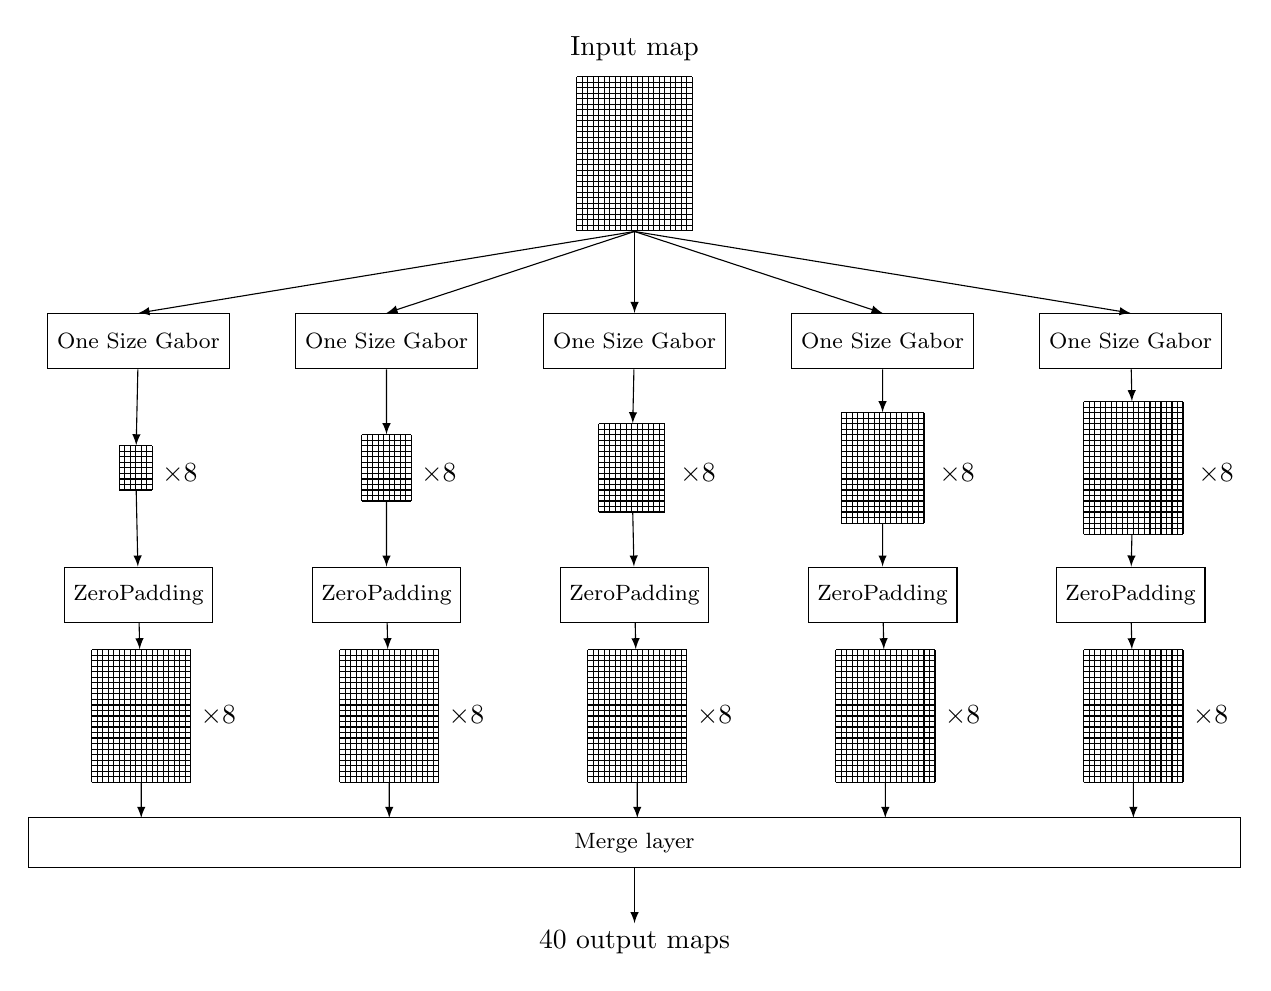
\begin{tikzpicture}[scale=\sfG,every path/.style={>=latex}]
		% draw input image
		\gridnode{inputimage}{9.5}{3}{2.1}{2.8}
		
		% draw one size gabor layers
		\foreach \x in {0,...,4}
		{
			\node (osg\x) at (\x * 4.5 + 1.55,1) [draw,rectangle,minimum height=1cm * \sfG] {\footnotesize One Size Gabor};
			\draw[->] (inputimage.south) to (osg\x.north);
		}
		
		% draw representatives for the 40 outputs
		\gridnode{r0}{1.2}{-1.7}{0.6}{0.8}
		\gridnode{r1}{5.6}{-1.9}{0.9}{1.2}
		\gridnode{r2}{9.9}{-2.1}{1.2}{1.6}
		\gridnode{r3}{14.3}{-2.3}{1.5}{2.0}
		\gridnode{r4}{18.7}{-2.5}{1.8}{2.4}
		
		% draw connections to the representatives and add $x8$
		\foreach \x in {0,...,4}
		{
			\draw[->] (osg\x) to (r\x);
			\node at (\x * 4.7 + 2.3,-1.4) {$\times 8$};
		}
		
		% draw zero padding layers
		\foreach \x in {0,...,4}{
			\node (zp\x) at (\x * 4.5 + 1.55,-3.6) [draw,rectangle,minimum height=1cm * \sfG] {\footnotesize ZeroPadding};
			\draw[->] (r\x) to (zp\x);
		}
		
		% draw zero-padded maps
		\foreach \x in {0,...,4}
		{
			\gridnode{zpm\x}{\x * 4.5 + 0.7}{-7}{1.8}{2.4}
			\draw[->] (zp\x) to (zpm\x);
			\node at (\x * 4.5 + 3,-5.8) {$\times 8$};
		}
		
		% draw merge layer
		\node (mergelayer) at (10.55,-8.1) [draw,rectangle,minimum width=22cm * \sfG,minimum height=0.9cm * \sfG] {\footnotesize Merge layer};
		
		% draw connections from zero padded maps to merge layer
		\foreach \x in {0,...,4}{	\draw[->] (zpm\x.south) to (\x * 4.5 + 1.6,-7.65);	}
		
		\draw[->] (mergelayer.south) -- ++(0,-1);
		\node at (10.55,-9.9) {40 output maps};
		\node at (10.55, 6.3) {Input map};
	\end{tikzpicture}
	\caption{The complete Gabor layer}
	\label{fig:complete_gabor_layer}
\end{figure}
